\section{DS1}
\subsection{Definition Biodiversität}
\textbf{Erste Nennung:} „National Forum of BioDiversity“ (Name einer Tagung 1986 in Washington, USA)\\
\textbf{Biodiversität = Information}\\
Components of biodiversity [nach Noss (1990)]
\begin{itemize}
	\item Compositional
	\begin{itemize}
		\item Genes
		\item Species, populations
		\item Communities/ecosystems
		\item Landscape type
	\end{itemize}
	\item Structural
	\begin{itemize}
		\item Landscape patterns
		\item Physiognomy/habitat structure
		\item Population structure
		\item Genetic structure
	\end{itemize}
	\item Functional
	\begin{itemize}
		\item Genetic process
		\item Demographic process
		\item Interspecific interactions
		\item Landscape process/disturbances
	\end{itemize}
\end{itemize}

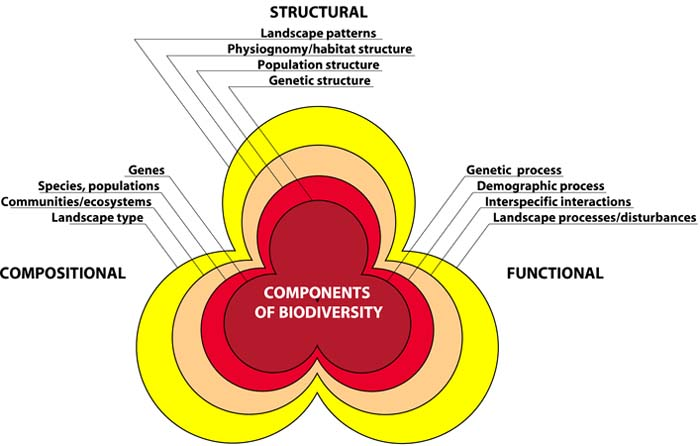
\includegraphics[width=0.8\textwidth]{lectures/DS1/pix/y5187e12.jpg}\\
http://www.fao.org/docrep/006/y5187e/y5187e12.jpg

\subsection{Facetten der Biodiversität}
\begin{itemize}
	\item Molekulare Vielfalt, z. B. Variation zwischen Proteinen (Isoenzyme)
	\item Chemische Vielfalt: z. B. Vielfalt der sekundären Inhaltsstoffe
	\item Genetische Vielfalt: z. B. Genotypen innerhalb einer Art
	\item Phylogenetische Vielfalt: Repräsentanz des „tree of life“
	\item Artenvielfalt: Anzahl und relative Abundanz von Arten
	\item Funktionelle Vielfalt: z. B. physiologische, anatomische, morphologische, demographische, ethologische Vielfalt
	\item Interaktionsvielfalt: z. B. Vielfalt der trophischen Beziehungen sowie aller Sym-, Pro- oder Antibiosen
	\item Ökosystemvielfalt: z. B. Vielfalt der Ökosysteme und Ökosystemprozesse in der Landschaft
\end{itemize}

\subsection{Entwicklung der Biodiversität}
Diversifizierungsmechanismen v.a. Meso-/Känozoische Radiation:
\begin{itemize}
	\item Nach Landgang in Silur zunehmende Nährstoffeinträge vom Land durch organische Partikel
	\item Auseinander brechen von Pangäa erhöht Klimagradienten, Nischenraum und schafft Verbreitungshindernisse, die die Entstehung von Endemismen begünstigen
	\item Zunehmen ausdifferenzierte Baupläne ermöglichen immer größere Spezialisierung und Ausnutzen ökologischer Nischen
\end{itemize}

\textbf{Sixth Mass Extinction:} \textcolor{red}{???}
\\

\textbf{Differentielle Entwicklung in Großtaxa:} Die jeweils neu entwickelten Taxa machen rasch die größte Diversität aus\\
Suche nach Asymptote: Anzahl der beschriebenen Arten über Jahre keine Asymptote $\rightarrow$ \textcolor{red}{Warum?}\\
Umso höher die Taxa umso weniger asymptotisch (Mora et al. 2011)\\

\newpage
\textbf{Wer ist wie häufig? (beschriebene Arten)}
\begin{itemize}
	\item 1.: Insekten $>$ 1 Mio.
	\item 2.: Pflanze $\sim$ 300000
	\item 12.: Vögel ca. 9950
	\item 18.: Amphibien ca. 4950
	\item 19.: Säugetiere ca. 4630
\end{itemize}

Pionier der Diversitätsforschung: Alexander von Humbolt beschreibt großräumige Diversitätsgradienten\\

erste globale Diversitätskarte: pflanzlichen Diversität nach Wulff (1935), aktualisiert von Mutke \& Barthlott (2005)